% ============================================================
% Question Bank: ch01-04 Writing Equations for Proportional Relationships
% Topic Title: Writing Equations for Proportional Relationships
% CCSS: 7.RP.A.2c
% Questions: 27 (15 MC + 6 SA + 6 Graphical)
% ============================================================

% --- Multiple Choice Questions (15) ---

\begin{practiceQuestion}{1-4-q01}{mc}
\begin{questionText}
A movie theater sells popcorn for $\$6.50$ per bag. Which equation represents the total cost $c$ for $b$ bags of popcorn?
\end{questionText}
\choiceA{$c = b + 6.50$}
\choiceB{$c = 6.50b$}
\choiceC{$c = \frac{b}{6.50}$}
\choiceD{$b = 6.50c$}
\correctAnswer{B}
\explanation{The cost is proportional to the number of bags at $\$6.50$ per bag. The equation is $c = kx$, so $c = 6.50b$.}
\end{practiceQuestion}

\begin{practiceQuestion}{1-4-q02}{mc}
\begin{questionText}
The table below shows a proportional relationship.

\begin{center}
\begin{tabular}{|c|c|}
\hline
$x$ & $y$ \\
\hline
$3$ & $13.5$ \\
$5$ & $22.5$ \\
$8$ & $36$ \\
\hline
\end{tabular}
\end{center}

Which equation represents this relationship?
\end{questionText}
\choiceA{$y = 3x$}
\choiceB{$y = 4x$}
\choiceC{$y = 4.5x$}
\choiceD{$y = 10.5x$}
\correctAnswer{C}
\explanation{Find $k$: $\frac{13.5}{3} = 4.5$. Check: $\frac{22.5}{5} = 4.5$ and $\frac{36}{8} = 4.5$. The equation is $y = 4.5x$.}
\end{practiceQuestion}

\begin{practiceQuestion}{1-4-q03}{mc}
\begin{questionText}
A swimming pool is being filled at a constant rate of $12.5$ gallons per minute. Which equation gives the total gallons $g$ after $m$ minutes?
\end{questionText}
\choiceA{$g = m + 12.5$}
\choiceB{$g = \frac{m}{12.5}$}
\choiceC{$m = 12.5g$}
\choiceD{$g = 12.5m$}
\correctAnswer{D}
\explanation{The total gallons equals the rate times the time: $g = 12.5m$. This is a proportional equation with $k = 12.5$.}
\end{practiceQuestion}

\begin{practiceQuestion}{1-4-q04}{mc}
\begin{questionText}
A landscaper earns $\$22$ per lawn. Using the equation $e = 22n$, how much does the landscaper earn after mowing $15$ lawns?
\end{questionText}
\choiceA{$\$220$}
\choiceB{$\$300$}
\choiceC{$\$330$}
\choiceD{$\$352$}
\correctAnswer{C}
\explanation{Substitute $n = 15$ into the equation: $e = 22 \times 15 = 330$. The landscaper earns $\$330$.}
\end{practiceQuestion}

\begin{practiceQuestion}{1-4-q05}{mc}
\begin{questionText}
A painter mixes paint using a ratio of $\frac{2}{3}$ cup of blue per cup of white. Which equation shows the relationship between cups of blue paint $b$ and cups of white paint $w$?
\end{questionText}
\choiceA{$b = \frac{3}{2}w$}
\choiceB{$b = \frac{2}{3}w$}
\choiceC{$b = w - \frac{2}{3}$}
\choiceD{$w = \frac{2}{3}b$}
\correctAnswer{B}
\explanation{For every $1$ cup of white, the painter uses $\frac{2}{3}$ cup of blue. The equation $b = \frac{2}{3}w$ shows blue as a function of white with $k = \frac{2}{3}$.}
\end{practiceQuestion}

\begin{practiceQuestion}{1-4-q06}{mc}
\begin{questionText}
A proportional relationship has the equation $y = 3.5x$. What is $x$ when $y = 28$?
\end{questionText}
\choiceA{$x = 4$}
\choiceB{$x = 8$}
\choiceC{$x = 24.5$}
\choiceD{$x = 31.5$}
\correctAnswer{B}
\explanation{Substitute $y = 28$: $28 = 3.5x$. Divide both sides by $3.5$: $x = \frac{28}{3.5} = 8$.}
\end{practiceQuestion}

\begin{practiceQuestion}{1-4-q07}{mc}
\begin{questionText}
On a farm, each chicken lays an average of $5$ eggs per week. Which equation represents the total number of eggs $e$ laid by $c$ chickens in one week?
\end{questionText}
\choiceA{$e = c + 5$}
\choiceB{$e = 5c$}
\choiceC{$c = 5e$}
\choiceD{$e = \frac{c}{5}$}
\correctAnswer{B}
\explanation{Each chicken lays $5$ eggs, so the total eggs equals $5$ times the number of chickens: $e = 5c$. This is a proportional equation with $k = 5$.}
\end{practiceQuestion}

\begin{practiceQuestion}{1-4-q08}{mc}
\begin{questionText}
A car's fuel efficiency is described by the equation $d = 28g$, where $d$ is distance in miles and $g$ is gallons of gas used. How many gallons are needed to travel $364$ miles?
\end{questionText}
\choiceA{$10$}
\choiceB{$13$}
\choiceC{$15$}
\choiceD{$336$}
\correctAnswer{B}
\explanation{Substitute $d = 364$: $364 = 28g$. Divide both sides by $28$: $g = \frac{364}{28} = 13$ gallons.}
\end{practiceQuestion}

\begin{practiceQuestion}{1-4-q09}{mc}
\begin{questionText}
From the table, a student writes the equation $y = 6x$. Which pair of values from the table confirms the equation?

\begin{center}
\begin{tabular}{|c|c|}
\hline
$x$ & $y$ \\
\hline
$2$ & $12$ \\
$4$ & $24$ \\
$7$ & $42$ \\
\hline
\end{tabular}
\end{center}
\end{questionText}
\choiceA{Only $(2, 12)$}
\choiceB{Only $(4, 24)$}
\choiceC{Only $(7, 42)$}
\choiceD{All three pairs}
\correctAnswer{D}
\explanation{Check each: $6 \times 2 = 12$ \checkmark, $6 \times 4 = 24$ \checkmark, $6 \times 7 = 42$ \checkmark. All three pairs satisfy $y = 6x$.}
\end{practiceQuestion}

\begin{practiceQuestion}{1-4-q10}{mc}
\begin{questionText}
A school orders $\frac{3}{4}$ pound of clay per student for an art project. Which equation gives the total pounds of clay $p$ needed for $s$ students?
\end{questionText}
\choiceA{$p = s + \frac{3}{4}$}
\choiceB{$p = \frac{4}{3}s$}
\choiceC{$p = \frac{3}{4}s$}
\choiceD{$s = \frac{3}{4}p$}
\correctAnswer{C}
\explanation{Each student needs $\frac{3}{4}$ pound, so total clay $= \frac{3}{4} \times$ students: $p = \frac{3}{4}s$.}
\end{practiceQuestion}

\begin{practiceQuestion}{1-4-q11}{mc}
\begin{questionText}
A runner's distance is modeled by $d = 7.5t$, where $d$ is in miles and $t$ is in hours. How far does the runner go in $2.5$ hours?
\end{questionText}
\choiceA{$10$ miles}
\choiceB{$15$ miles}
\choiceC{$18.75$ miles}
\choiceD{$20$ miles}
\correctAnswer{C}
\explanation{Substitute $t = 2.5$: $d = 7.5 \times 2.5 = 18.75$ miles.}
\end{practiceQuestion}

\begin{practiceQuestion}{1-4-q12}{mc}
\begin{questionText}
A plumber charges $\$45$ per hour with no service fee. If the total cost was $\$247.50$, how many hours did the plumber work?
\end{questionText}
\choiceA{$4.5$ hours}
\choiceB{$5$ hours}
\choiceC{$5.5$ hours}
\choiceD{$6$ hours}
\correctAnswer{C}
\explanation{Write the equation $c = 45h$. Substitute $c = 247.50$: $247.50 = 45h$, so $h = \frac{247.50}{45} = 5.5$ hours.}
\end{practiceQuestion}

\begin{practiceQuestion}{1-4-q13}{mc}
\begin{questionText}
Tyler says the equation for the table below is $y = 8x$.

\begin{center}
\begin{tabular}{|c|c|}
\hline
$x$ & $y$ \\
\hline
$5$ & $40$ \\
$9$ & $72$ \\
$11$ & $88$ \\
\hline
\end{tabular}
\end{center}

Is Tyler correct?
\end{questionText}
\choiceA{Yes, because $40 \div 5 = 8$}
\choiceB{No, because $88 \div 11 = 9$}
\choiceC{No, because $72 \div 9 = 7$}
\choiceD{Yes, because $72 \div 9 = 8$ and $88 \div 11 = 8$}
\correctAnswer{D}
\explanation{Check every row: $40 \div 5 = 8$, $72 \div 9 = 8$, $88 \div 11 = 8$. All ratios equal $8$, confirming the equation $y = 8x$. Tyler is correct.}
\end{practiceQuestion}

\begin{practiceQuestion}{1-4-q14}{mc}
\begin{questionText}
A caterer uses $1.5$ pounds of rice per guest. How many guests can be served with $48$ pounds of rice?
\end{questionText}
\choiceA{$24$}
\choiceB{$32$}
\choiceC{$46.5$}
\choiceD{$72$}
\correctAnswer{B}
\explanation{Write the equation $r = 1.5g$. Substitute $r = 48$: $48 = 1.5g$, so $g = \frac{48}{1.5} = 32$ guests.}
\end{practiceQuestion}

\begin{practiceQuestion}{1-4-q15}{mc}
\begin{questionText}
Which equation does \textbf{not} represent a proportional relationship?
\end{questionText}
\choiceA{$y = 9x$}
\choiceB{$y = \frac{1}{4}x$}
\choiceC{$y = 5x + 3$}
\choiceD{$y = 0.6x$}
\correctAnswer{C}
\explanation{A proportional equation must have the form $y = kx$ with no added constant. Choice C has "$+ 3$," which is a $y$-intercept that prevents the graph from passing through the origin.}
\end{practiceQuestion}

% --- Short Answer Questions (6) ---

\begin{practiceQuestion}{1-4-q16}{sa}
\begin{questionText}
A printer prints $18$ pages per minute. Write the equation for the number of pages $p$ printed in $m$ minutes.
\end{questionText}
\correctAnswer{$p = 18m$}
\explanation{The unit rate is $18$ pages per minute, so the equation is $p = 18m$. Substitute any value of $m$ to find the total pages.}
\end{practiceQuestion}

\begin{practiceQuestion}{1-4-q17}{sa}
\begin{questionText}
Using the equation $y = 3.2x$, find $y$ when $x = 25$.
\end{questionText}
\correctAnswer{$80$}
\explanation{Substitute $x = 25$: $y = 3.2 \times 25 = 80$.}
\end{practiceQuestion}

\begin{practiceQuestion}{1-4-q18}{sa}
\begin{questionText}
A store sells trail mix for $\$4.80$ per pound. How much do $3.5$ pounds cost?
\end{questionText}
\correctAnswer{$\$16.80$}
\explanation{Write the equation $c = 4.80p$. Substitute $p = 3.5$: $c = 4.80 \times 3.5 = 16.80$. The cost is $\$16.80$.}
\end{practiceQuestion}

\begin{practiceQuestion}{1-4-q19}{sa}
\begin{questionText}
The equation $d = 55t$ models a car's trip, where $d$ is distance in miles and $t$ is time in hours. How many hours does it take to travel $385$ miles?
\end{questionText}
\correctAnswer{$7$}
\explanation{Substitute $d = 385$: $385 = 55t$, so $t = \frac{385}{55} = 7$ hours.}
\end{practiceQuestion}

\begin{practiceQuestion}{1-4-q20}{sa}
\begin{questionText}
Write an equation for the proportional relationship shown in the table.

\begin{center}
\begin{tabular}{|c|c|}
\hline
$x$ & $y$ \\
\hline
$6$ & $15$ \\
$10$ & $25$ \\
\hline
\end{tabular}
\end{center}
\end{questionText}
\correctAnswer{$y = 2.5x$}
\explanation{Find $k$: $\frac{15}{6} = 2.5$. Check: $\frac{25}{10} = 2.5$. The equation is $y = 2.5x$.}
\end{practiceQuestion}

\begin{practiceQuestion}{1-4-q21}{sa}
\begin{questionText}
An orchard sells apples at a constant price. If $8$ apples cost $\$6.00$, how much do $20$ apples cost?
\end{questionText}
\correctAnswer{$\$15.00$}
\explanation{Find the unit price: $k = \frac{6.00}{8} = 0.75$ per apple. Write the equation $c = 0.75a$. Substitute $a = 20$: $c = 0.75 \times 20 = 15.00$.}
\end{practiceQuestion}

% --- Graphical Multiple Choice Questions (3) ---

\begin{practiceQuestion}{1-4-q22}{gmc}
\begin{questionText}
The graph below shows a proportional relationship between hours worked and money earned.

\begin{center}
\begin{tikzpicture}[scale=0.5]
  \draw[step=1,gray!20,thin] (0,0) grid (8,10);
  \draw[thick,->] (0,0) -- (8.5,0) node[right]{\small Hours};
  \draw[thick,->] (0,0) -- (0,10.5) node[above]{\small Earnings (\$)};
  \foreach \x in {1,...,8} \draw (\x,0.1) -- (\x,-0.1) node[below]{\tiny \x};
  \foreach \y in {1,...,10} \draw (0.1,\y) -- (-0.1,\y) node[left]{\tiny \y};
  \draw[thick,funBlue] (0,0) -- (8,10);
  \fill[funBlue] (0,0) circle (3pt);
  \fill[funBlue] (4,5) circle (3pt);
  \fill[funBlue] (8,10) circle (3pt);
\end{tikzpicture}
\end{center}

Which equation represents this graph?
\end{questionText}
\choiceA{$e = 0.8h$}
\choiceB{$e = 1.25h$}
\choiceC{$e = 5h$}
\choiceD{$e = 2h$}
\correctAnswer{B}
\explanation{From the graph, the point $(4, 5)$ gives $k = \frac{5}{4} = 1.25$. The equation is $e = 1.25h$.}
\end{practiceQuestion}

\begin{practiceQuestion}{1-4-q23}{gmc}
\begin{questionText}
The table below shows the cost of renting kayaks for different numbers of hours.

\begin{center}
\begin{tabular}{|c|c|}
\hline
\textbf{Hours} & \textbf{Cost (\$)} \\
\hline
$1$ & $\$14$ \\
$3$ & $\$42$ \\
$5$ & $\$70$ \\
$h$ & $?$ \\
\hline
\end{tabular}
\end{center}

Which equation can be used to find the cost for any number of hours $h$?
\end{questionText}
\choiceA{$c = h + 14$}
\choiceB{$c = 14h$}
\choiceC{$c = 28h$}
\choiceD{$c = 7h$}
\correctAnswer{B}
\explanation{Find $k$: $14 \div 1 = 14$, $42 \div 3 = 14$, $70 \div 5 = 14$. The constant of proportionality is $14$, so $c = 14h$.}
\end{practiceQuestion}

\begin{practiceQuestion}{1-4-q24}{gmc}
\begin{questionText}
The double number line below shows the proportional relationship between liters of paint and square meters covered.

\begin{center}
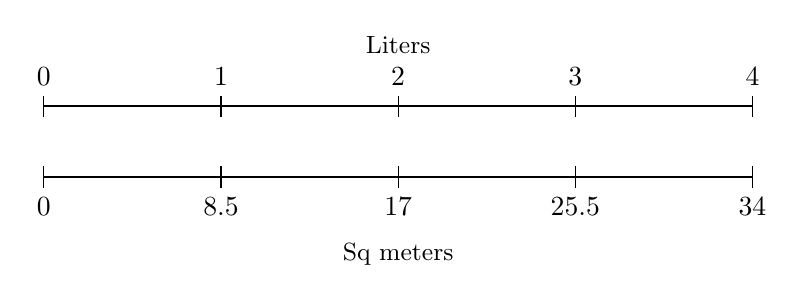
\begin{tikzpicture}[scale=0.9]
  \draw[thick] (0,0.5) -- (10,0.5);
  \draw[thick] (0,-0.5) -- (10,-0.5);
  \foreach \x/\lab in {0/0, 2.5/1, 5/2, 7.5/3, 10/4}
    \draw (\x,0.35) -- (\x,0.65) node[above]{$\lab$};
  \node[above] at (5,1.1) {\small Liters};
  \foreach \x/\lab in {0/0, 2.5/8.5, 5/17, 7.5/25.5, 10/34}
    \draw (\x,-0.35) -- (\x,-0.65) node[below]{$\lab$};
  \node[below] at (5,-1.3) {\small Sq meters};
\end{tikzpicture}
\end{center}

Which equation represents the relationship?
\end{questionText}
\choiceA{$s = 8.5l$}
\choiceB{$l = 8.5s$}
\choiceC{$s = l + 8.5$}
\choiceD{$s = 4.25l$}
\correctAnswer{A}
\explanation{From the double number line, $1$ liter covers $8.5$ sq meters. The equation is $s = 8.5l$. Check: $2$ liters covers $8.5 \times 2 = 17$ \checkmark.}
\end{practiceQuestion}

% --- Graphical Short Answer Questions (3) ---

\begin{practiceQuestion}{1-4-q25}{gsa}
\begin{questionText}
The graph below shows a proportional relationship.

\begin{center}
\begin{tikzpicture}[scale=0.5]
  \draw[step=1,gray!20,thin] (0,0) grid (10,8);
  \draw[thick,->] (0,0) -- (10.5,0) node[right]{$x$};
  \draw[thick,->] (0,0) -- (0,8.5) node[above]{$y$};
  \foreach \x in {2,4,...,10} \draw (\x,0.1) -- (\x,-0.1) node[below]{\tiny \x};
  \foreach \y in {1,...,8} \draw (0.1,\y) -- (-0.1,\y) node[left]{\tiny \y};
  \draw[thick,funOrange] (0,0) -- (10,6);
  \fill[funOrange] (0,0) circle (3pt);
  \fill[funOrange] (5,3) circle (3pt);
  \fill[funOrange] (10,6) circle (3pt);
\end{tikzpicture}
\end{center}

Write the equation for this proportional relationship.
\end{questionText}
\correctAnswer{$y = 0.6x$}
\explanation{From the graph, the point $(5, 3)$ gives $k = \frac{3}{5} = 0.6$. The equation is $y = 0.6x$. Check: $0.6 \times 10 = 6$ \checkmark.}
\end{practiceQuestion}

\begin{practiceQuestion}{1-4-q26}{gsa}
\begin{questionText}
The table below shows a proportional relationship between the number of hours and the distance walked.

\begin{center}
\begin{tabular}{|c|c|}
\hline
\textbf{Hours} ($t$) & \textbf{Miles} ($d$) \\
\hline
$2$ & $7$ \\
$4$ & $14$ \\
$6$ & $21$ \\
\hline
\end{tabular}
\end{center}

Write the equation, and use it to find how far the person walks in $9$ hours.
\end{questionText}
\correctAnswer{$31.5$ miles}
\explanation{Find $k = \frac{7}{2} = 3.5$. The equation is $d = 3.5t$. Substitute $t = 9$: $d = 3.5 \times 9 = 31.5$ miles.}
\end{practiceQuestion}

\begin{practiceQuestion}{1-4-q27}{gsa}
\begin{questionText}
A proportional graph passes through the points shown below.

\begin{center}
\begin{tikzpicture}[scale=0.45]
  \draw[step=1,gray!20,thin] (0,0) grid (10,10);
  \draw[thick,->] (0,0) -- (10.5,0) node[right]{$x$};
  \draw[thick,->] (0,0) -- (0,10.5) node[above]{$y$};
  \foreach \x in {1,...,10} \draw (\x,0.1) -- (\x,-0.1) node[below]{\tiny \x};
  \foreach \y in {1,...,10} \draw (0.1,\y) -- (-0.1,\y) node[left]{\tiny \y};
  \draw[thick,funPurple] (0,0) -- (10,7.5);
  \fill[funPurple] (0,0) circle (3pt);
  \fill[funPurple] (4,3) circle (3pt);
  \fill[funPurple] (8,6) circle (3pt);
\end{tikzpicture}
\end{center}

Write the equation, and find the value of $y$ when $x = 14$.
\end{questionText}
\correctAnswer{$10.5$}
\explanation{From the point $(4, 3)$: $k = \frac{3}{4} = 0.75$. The equation is $y = 0.75x$. Substitute $x = 14$: $y = 0.75 \times 14 = 10.5$.}
\end{practiceQuestion}
